\documentclass[a4paper]{article}
\usepackage{vntex}
\usepackage{listings}
%\usepackage[english,vietnam]{babel}
%\usepackage[utf8]{inputenc}

%\usepackage[utf8]{inputenc}
%\usepackage[francais]{babel}
\usepackage{a4wide,amssymb,epsfig,latexsym,array,hhline,fancyhdr}

\usepackage{amsmath}
\usepackage{amsthm}
\usepackage{multicol,longtable,amscd}
\usepackage{diagbox}%Make diagonal lines in tables
\usepackage{booktabs}
\usepackage{alltt}
\usepackage[framemethod=tikz]{mdframed}% For highlighting paragraph backgrounds
\usepackage{caption,subcaption}

\usepackage{lastpage}
\usepackage[lined,boxed,commentsnumbered]{algorithm2e}
\usepackage{enumerate}
\usepackage{color}
\usepackage{graphicx}							% Standard graphics package
\usepackage{array}
\usepackage{tabularx, caption}
\usepackage{multirow}
\usepackage{multicol}
\usepackage{rotating}
\usepackage{graphics}
\usepackage{geometry}
\usepackage{setspace}
\usepackage{epsfig}
\usepackage{tikz}
\usetikzlibrary{arrows,snakes,backgrounds}
\usepackage[unicode]{hyperref}
\hypersetup{urlcolor=blue,linkcolor=black,citecolor=black,colorlinks=true} 
%\usepackage{pstcol} 								% PSTricks with the standard color package

\newtheorem{theorem}{{\bf Định lý}}
\newtheorem{property}{{\bf Tính chất}}
\newtheorem{proposition}{{\bf Mệnh đề}}
\newtheorem{corollary}[proposition]{{\bf Hệ quả}}
\newtheorem{lemma}[proposition]{{\bf Bổ đề}}

\everymath{\color{blue}}%make in-line maths symbols blue to read/check easily
\definecolor{dkgreen}{rgb}{0,0.6,0}
\definecolor{gray}{rgb}{0.5,0.5,0.5}
\definecolor{mauve}{rgb}{0.58,0,0.82}
\lstset{frame=tb,
  language=R,
  aboveskip=3mm,
  belowskip=3mm,
  showstringspaces=false,
  columns=flexible,
  basicstyle={\small\ttfamily},
  numbers=none,
  numberstyle=\tiny\color{gray},
  keywordstyle=\color{blue},
  commentstyle=\color{dkgreen},
  stringstyle=\color{mauve},
  breaklines=true,
  breakatwhitespace=true,
  tabsize=3
}

\usepackage[utf8]{inputenc}

\title{Sir roi rac version2}
\author{lephongplus2016 }
\date{July 2020}

\begin{document}

\maketitle

\section{Introduction}
\subsection{Trường hợp rời rạc} Trường hợp rời rạc của mô hình SIR là hệ phương trình sai phân sau:
\begin{align*} 
    &R(n+1) 	= R(n) + \gamma (\Delta t) I(n)  \\
	&I(n+1) 	= I(n) - \gamma (\Delta t) I(n) + \beta (\Delta t) I(n)S(n)   \\
	&S(n+1) 	= S(n) - \beta (\Delta t) S(n)I(n)  \label{eq3}
	\end{align*}
	Với $ S_{0}>0 $,$ I_{0}>0 $,$ R_{0}>0 $, ta có thỏa mãn tính chất sau: 
	$ S_{0} + I_{0} + R_{0} = N $ \\
		\begin{itemize}
	\item $S(n)$ : Số người có nguy cơ mắc bệnh;
	\item $I(n)$ : Số người bị nhiễm bệnh;
	\item $R(n)$ : Số người hồi phục sau bệnh;
	\item $\beta(n)$ : Tỷ lệ tiếp xúc của người trong nhóm $S(t)$ với người trong nhóm $I(n)$, được tính dựa trên các yếu tố thực tế như bán kính đi lại, mức độ tiếp xúc giữa người mắc bệnh với người có khả năng mắc bệnh, tính chất của virus,...;
	\item $\gamma(n)$ : Tỷ lệ hồi phục khi mắc bệnh, được tính bằng cách lấy 1 chia cho khoảng thời gian trung bình mà một người phục hồi;
	\item $N(n)$ : Tổng số người trong cộng đồng cách ly;
	\end{itemize}
	Giả sử rằng $\beta$ , $\gamma$ là các giá trị không đổi và có thể xác định từ các dữ liệu ban đầu. Các cá nhân phục hồi từ căn bệnh sẽ trở miễn dịch vĩnh viễn.\\
	Trong hệ rời rạc chỉ xét số nguyên dương cho n=1,2,... .\\
	
	
	Ta có hệ các phương trình thể hiện tốc độ thay đổi $ S$,   $I $, $ R$:
	\begin{align*} 
    &R^{'} 	= \gamma (\Delta t) I  \\
	&I^{'} 	= - \gamma (\Delta t) I + \beta (\Delta t) IS   \\
	&S^{'} 	= - \beta (\Delta t) SI  \label{eq3}
	\end{align*}
    Giới hạn của $S$ thì phụ thuộc vào các điều kiện ban đầu\\ Nếu $S_{0} \leq \frac{\gamma}{\beta} $, thì $I_{1} \leq I_{0}$ và $S_{n}$ giảm dần $I_{n+1} \leq I_{n}$ hay $I^{'}<0$; Không còn dịch bệnh.\\
	Ngược lại, nếu $S_{0} > \frac{\gamma}{\beta} $, thì $I_{1} > I_{0}$ hay $I^{'}>0$ nhóm người bị nhiễm bệnh đang gia tăng.\\

\section{Bài toán 3}
Nhóm chọn ngôn ngữ thống kê R để thực hiện bài toán.\\

Mô tả cách thiết lập và chạy Metropolis-Hastings dựa trên Markov chain Monte Carlo (MCMC) trong phạm vi mô hình SIR.\\
Ví dụ code sử dụng dữ liệu Eyam.\\
\begin{lstlisting}

library(MultiBD)

data(Eyam)

print(Eyam)

printsample_size <- 177
\end{lstlisting}
\\
Tính log của phân bố xác suất số ca mắc bệnh và số người có khả năng mắc bệnh với param cho trước. Ma trận xác suất được trả về bởi $ ddb_{-}prob() $ tương ứng với giá trị $S$ từ $a$ tới $a_{0}$  và $I$ từ $0$ tới $B$.\\
$a$ là cận dưới, $B$ là cận trên.
\\
$ ddb_{-}prob() $ Function là Xác suất chuyển tiếp của một quá trình chết/ sinh - chết..\\
\lstinline{drates1} Tỉ lệ chết đi của $S$, bằng 0 vì $S$ chỉ chuyển số lượng sang cho $I$.\\
\lstinline{brates2} Mô hình không sinh thêm phần tử.\\
\lstinline{drates2} Tỉ lệ chết của $I$ là có và bằng \lstinline{alpha*b}.\\
\lstinline{trans12} Ở đây là mô hình chuyển từ trạng thái $S$ sang trạng thái $I$
\\
\begin{lstlisting}

loglik_sir <- function(param, data) {
                                            
  alpha <- exp(param[1]) # Rates must be non-negative
  beta <- exp(param[2])
  # Set-up SIR model
  drates1 <- function(a, b) { 0 }                    
  brates2 <- function(a, b) { 0 }                     
  drates2 <- function(a, b) { alpha * b }            
  trans12 <- function(a, b) { beta * a * b }          
  sum(sapply(1:(nrow(data) - 1), # Sum across all time steps k
             function(k) {
               log( # sums the logs of logs that change from T to T + 1 state
                 dbd_prob( # Compute the transition probability matrix
                   t = data$time[k + 1] - data$time[k], # Time increment
                   a0 = data$S[k], b0 = data$I[k], # From: S(t_k), I(t_k)
                   drates1, brates2, drates2, trans12,
                   a = data$S[k + 1], B = data$S[k] + data$I[k] - data$S[k + 1],
                   computeMode = 4, nblocks = 80 # Compute using 4 threads
                 )[1, data$I[k + 1] + 1] # To: S(t_(k+1)), I(t_(k+1))
               )
             }))
}
\end{lstlisting}
\\
Phân bố xác suất tiên nghiệm của số ca mắc bệnh và số ca phục hồi dựa trên phân bố chuẩn.

\\
\begin{lstlisting}
logprior <- function(param) { 
  log_alpha <- param[1]
  log_beta <- param[2]
  dnorm(log_alpha, mean = 0, sd = 100, log = TRUE) +
    dnorm(log_beta, mean = 0, sd = 100, log = TRUE)
}

library(MCMCpack)

alpha0 <- 3.39
beta0 <- 0.0212

post_sample <- MCMCmetrop1R(fun = function(param) { loglik_sir(param, Eyam) + logprior(param) },
                            theta.init = log(c(alpha0, beta0)),
                            mcmc = 177, burnin = 50)
# Sampling of beta, gamm

\end{lstlisting}
\\
Vẽ đồ thị minh họa:
\\
\begin{lstlisting}
plot(as.vector(post_sample[,1]), type = "l", xlab = "Iteration", ylab = expression(log(alpha)))

plot(as.vector(post_sample[,2]), type = "l", xlab = "Iteration", ylab = expression(log(beta)))


R_0 <- 0 
for(i in 1:8){
   R_0 <- R_0 + exp(loglik_sir(c(post_sample[i,1], post_sample[i,2]), Eyam))*(exp(post_sample[i,1])/exp(post_sample[i,2]))
}

print(R_0)




\end{lstlisting}

\\
\begin{center}
    \begin{figure}[htp]
    \begin{center}
     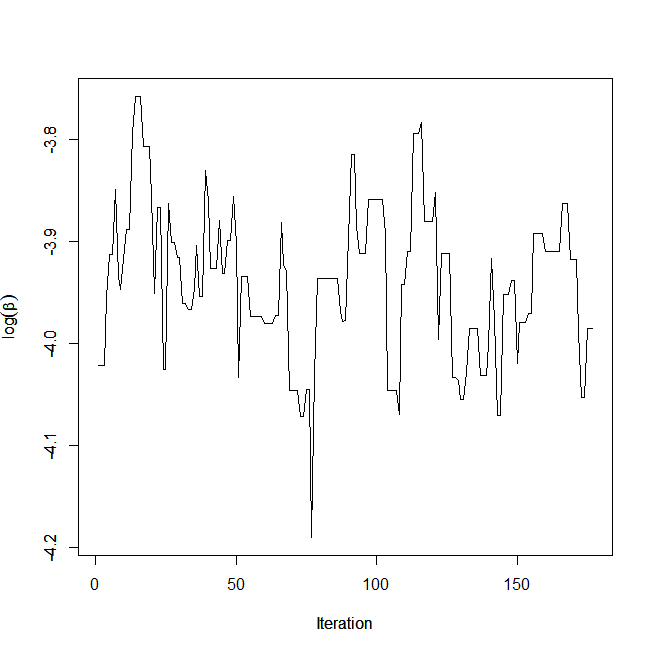
\includegraphics[scale=.5]{Images/Sir1.png}
    \end{center}
    \caption{Đồ thị minh họa}
    \label{refhinh1}
    \end{figure}
\end{center}

Kết quả tính được với ví dụ trên là :
\lstinline{The Metropolis acceptance rate was 0.51542}\\
$R_{0}$ là 1.543797e-15.

\end{document}
